\chapter{Introduction}
\label{ch:introduction}

\section{Background}
\label{sec:background}

Air pollution is now one of the biggest single environmental risk factors to human health globally, and its burden falls disproportionately on rapidly industrializing, low- and middle-income countries. The 2021 revision of the World Health Organization’s global air quality guidelines lowered the recommended annual mean PM2.5 exposure limit from 10 $\mu$g/m$^3$ to 5 $\mu$g/m$^3$, a change motivated in part by evidence that even the non-anthropogenic (natural) background component of PM2.5 in many regions already approaches this stricter limit, leaving almost no safe margin for additional anthropogenic (human-caused) emissions \citep{pai2022who}. This old, less stringent guideline has been difficult to meet for small and medium-sized industrial cities in developing economies, let alone the tightened 2021 target \citep{polezer2023new}.

Bangladesh is repeatedly ranked as one of the most affected countries by ambient and occupational air pollution. At the national level, evidence papers identify dominant factors for the air quality crisis in the country such as vehicular emissions, brick kilns, and unplanned industrial growth, with already significant and escalating health, productivity, and economic consequences \citep{khatun2023evidence}. Long-term satellite and ground-based re- constructions of PM2.5 over Bangladesh confirm the existence of persistent, spatially concentrated pollution hot spots rather than a uniform national exposure level, with some industrial districts consistently showing the highest sustained concentrations and associated health risk \citep{ali2025longterm}. City-specific studies at finer spatial resolution support this picture. Work in the Tejgaon industrial area of Dhaka reports PM2.5 and PM10 concentrations, and associated health risk indices, that vary sharply across relatively short distances depending on proximity to specific industrial sources \citep{basak2025spatial}. Satellite-based trend analysis of Chattogram similarly finds that the country’s second-largest industrial hub remains comparatively understudied despite clear pollutant loading \citep{huraira2024spatial}. This body of work collectively supports a central premise of the present capstone project: industrial air pollution in Bangladesh is not uniform across a city or a factory compound, but is concentrated at certain hotspots and the workers placed at those hotspots bear a disproportionate share of the exposure.

\subsection{Industrial Pollution in Bangladesh}
\label{sec:industrial-pollution-bd}

Plant engineers are familiar with point sources of hazardous air pollutants within individual industrial facilities, even if not formally instrumented. Welding stations emit metal-fume particulates and ozone; boiler rooms and generator rooms emit combustion by-products including CO, NO2, and smoke; chemical storage and handling areas emit VOCs and, depending on the process, NH3 or H2S; and factory entrances and loading zones accumulate vehicular and dust emissions.\
The health burden is documented directly in occupational-exposure studies at similar industrial facilities elsewhere: fibre-cement roofing workers exposed to elevated PM2.5 demonstrate measurable lung function impairment \citep{nasri2023pm25}, construction-site workers exposed to particulate matter show a range of associated health effects \citep{sekhavati2023particulate}, and broader reviews link chronic occupational PM2.5 exposure to elevated risk of mental health conditions including depression and anxiety-spectrum disorders, in addition to the well-established respiratory and cardiovascular effects \citep{alhadhrami2024pm25mental}. In Bangladesh specifically, industrial effluent and emissions from sources near Dhaka have been shown to increase trace-element and particulate loading in the surrounding environments to levels of ecological and health concern \citep{lisa2025investigative}, and even routine urban exposure is associated with measurable self-reported health deterioration in the general population of pollution-prone areas \citep{rahman2025perceived}.

Despite this evidence, the dominant response to industrial air pollution in Bangladesh – where it exists at all – is regulatory monitoring at coarse spatial and temporal reso- lution, or, at best, general ventilation and personal protective equipment (PPE) at the factory level. Centralized, plant-wide or city-wide air purification is prohibitively ex- pensive for the vast majority of small and medium enterprises that make up the bulk of the country’s manufacturing base, and even where affordable purification technology exists, adoption is limited. Field evidence from Dhaka households shows that willing- ness to pay for air purifiers is far below their real cost, driven partly by misbeliefs about indoor air quality and about purifier effectiveness \citep{chowdhury2025misbeliefs}. This mix of high point-source exposure, well-documented health consequences and low economic feasibility of conventional whole-space purification is the particular gap that motivates the system proposed in this capstone.

\begin{figure}[htbp]
    \centering
    \begin{minipage}[t]{0.48\textwidth}
        \centering
        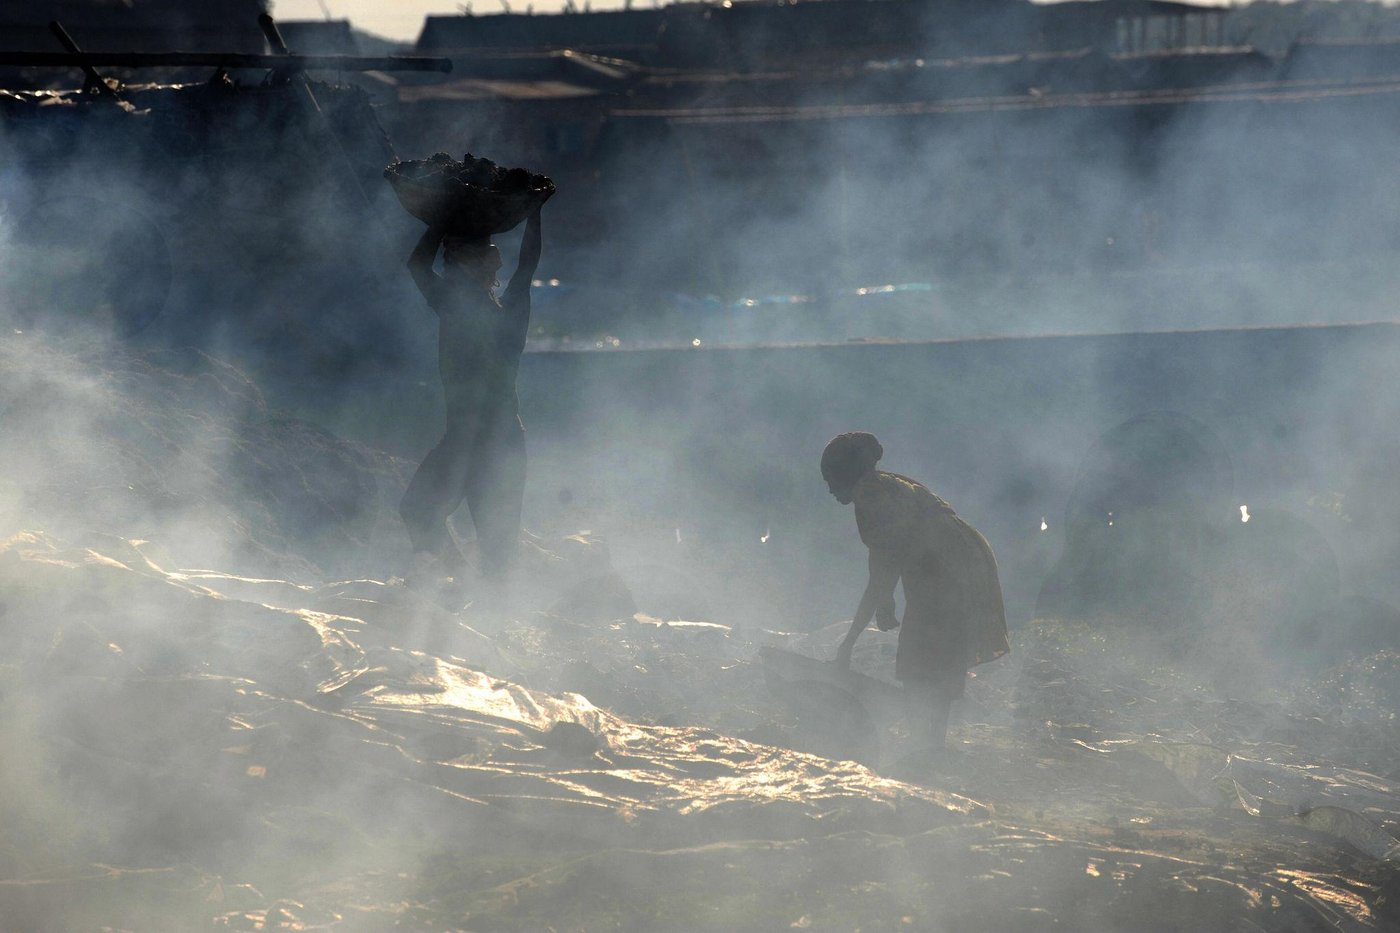
\includegraphics[width=\linewidth]{figures/hotspot_smoke.jpg}
    \end{minipage}
    \hfill
    \begin{minipage}[t]{0.48\textwidth}
        \centering
        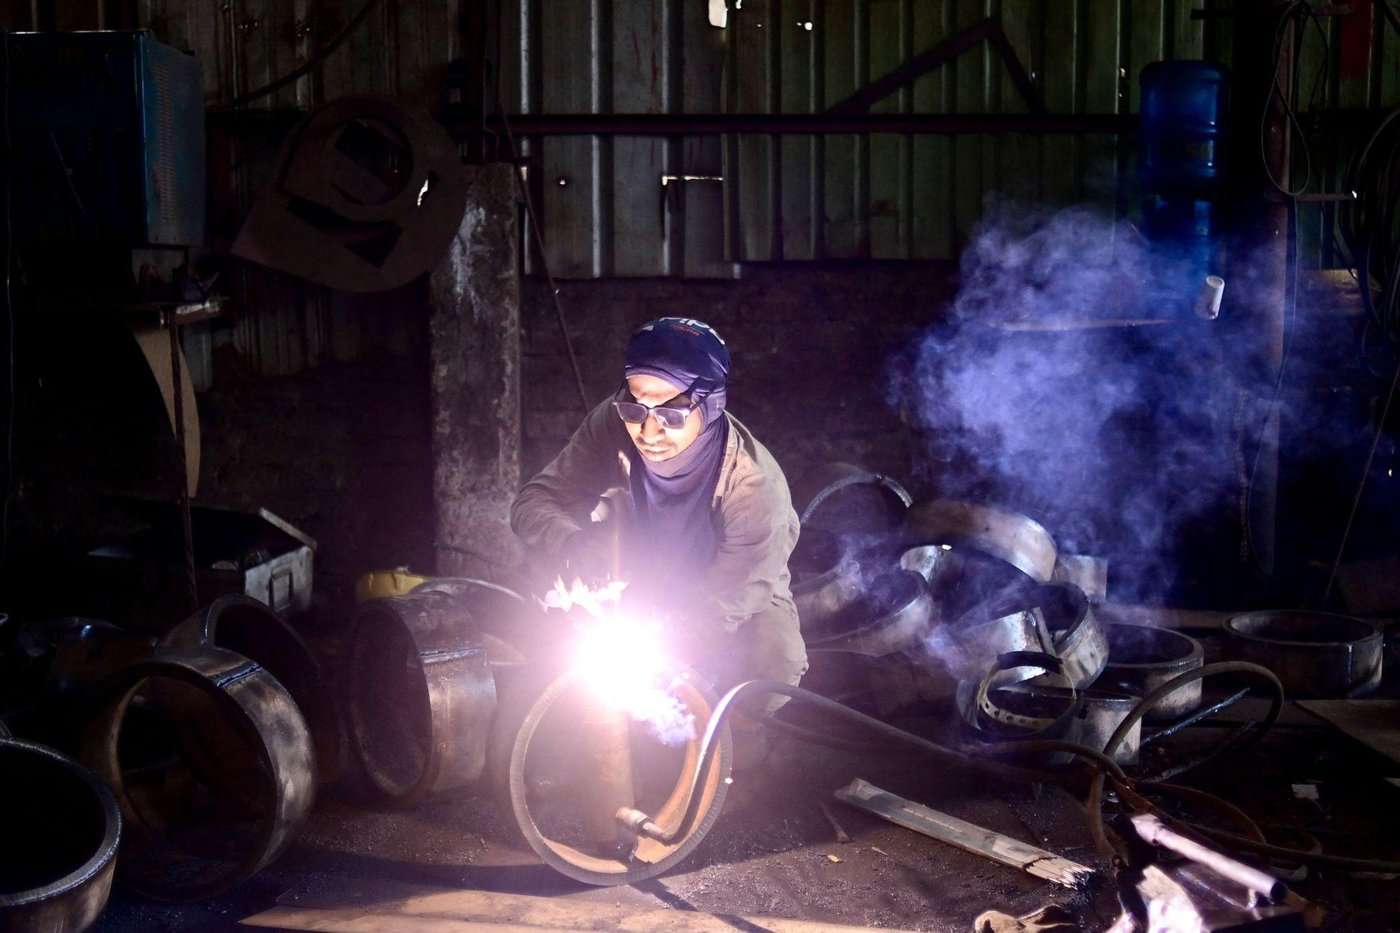
\includegraphics[width=\linewidth]{figures/hotspot_welding.jpg}
    \end{minipage}
    \caption{Representative industrial hotspots illustrating localized worker exposure to airborne pollution, including heavy smoke exposure and welding fumes.}
    \label{fig:hotspot-photo}
\end{figure}

\section{Problem Statement}
\label{sec:problem-statement}

There are three significant limitations of the existing air quality management approaches for the industrial settings of Bangladesh:

\begin{enumerate}[label=(\roman*)]
    \item Misalignment in space Air quality monitoring and purification are often conceived of at city or plant level whereas hazardous exposure is focused on certain micro-locations (welding bays, boiler rooms, chemical stores) that a coarse-grained system cannot target specifically.
    
    \item Response is reactive, not predictive. Conventional systems, where available at all, provide current pollutant levels, rather than predictions of near-future levels, so that any mitigating action (ventilation, evacuation, purification) can only begin after hazardous conditions have developed.
    
    \item Non-adaptive, static intelligence. The machine learning algorithms implemented in the current air-quality prediction systems are typically trained once on a fixed historical dataset and are not equipped to keep learning from the particular site where they are deployed. Thus, their accuracy degrades when the conditions are different from the training distribution or when the unit is relocated to a new site.
    
    \item large scale cost and energy infeasibility Deploying and retraining full-scale purification units and conventional deep-learning-based prediction pipelines over the large number of small industrial hotspots that would need to be covered in a realistic national deployment is computationally and financially costly.
\end{enumerate}

\section{Motivation}
\label{sec:motivation}

The motivation for this work follows immediately from the above problem statement. If hazardous exposure is concentrated at specific identifiable hotspots, then the most resource efficient mitigation strategy is not to purify an entire factory floor or an entire city, but to purify the small air volume immediately surrounding an exposed worker, and only at the moments when it is actually needed. This is directly analogous to the “Green” computing philosophy underlying energy-aware embedded systems and lightweight machine learning: to expend only the energy, compute, and material resources that a task genuinely requires, avoiding the overhead of solutions engineered for a much larger and more expensive scale.

Independent evidence from the portable/room air-purifier literature supports the technical feasibility of this localized approach: HEPA-based portable purifiers have been demonstrated to significantly reduce indoor particulate matter concentrations in real-world conditions \citep{lu2023realworld,cox2018effectiveness}, HEPA filtration improves indoor PM2.5 levels measurably in enclosed environments such as vehicles and public busses \citep{lee2022effect,chen2022efficacy}, and combined mechanical filtration (HEPA plus supplementary stages) has been shown to be more effective than ionization-based approaches for particulate removal \citep{dubey2021assessing,szczotko2022review}. Portable HEPA filtration has demonstrated the ability to effectively decrease indoor PM2.5 exposure even during severe pollution events, such as those associated with wildfire smoke \citep{chen2025fine}. These findings, based on purifiers for enclosed spaces at room- or vehicle-scale, motivate the extension of the same filtration principle -- cyclone pre-separation, HEPA filtration and activated-carbon adsorption -- to a compact, localized, worker-facing unit rather than a room-scale appliance.

In terms of prediction, earlier IoT-based air quality systems have shown that low-cost microcontrollers and commodity gas/particulate sensors can be used to build functioning real-time monitoring networks \citep{alam2025iot,zhang2020realtime,kataria2022aiiot,mani2021aipowered}, and that low-cost sensor networks are a practical and increasingly indispensable tool for air quality management particularly in developing-country settings with scarce reference-grade monitoring infrastructure \citep{shabbir2025paradigm}. This capstone addresses directly what is relatively underexplored in this literature, i.e. the combination of (a) hyper-local, hotspot-targeted purification, (b) short-horizon (1--2 hour) predictive activation rather than reactive activation, and (c) continuous, incremental, area-specific model adaptation after deployment.

\section{Research Gap}
\label{sec:research-gap}

Chapter 2 provides a detailed literature review. The main gap that this capstone aims to fill can be summarized as follows. The reviewed literature, (i) IoT based air quality monitoring, (ii) AI based pollution prediction and (iii) portable/indoor air purification address each one of the aspects of the problem in isolation. Pollutant levels are reported or forecasted in monitoring and prediction systems \citep{alam2025iot,zhang2020realtime,kataria2022aiiot,mani2021aipowered,islam2025dhaka}, but generally not coupled to an automated, localized purification response. Studies on purification effectiveness \citep{dubey2021assessing,lu2023realworld,cox2018effectiveness,chen2022efficacy,lee2022effect,chen2025fine,szczotko2022review} assess air cleaners as room-scale or vehicle-scale appliances rather than as hotspot-targeted, worker-proximate units, and are typically evaluated with reactive (current-condition) rather than predictive control. Health and exposure studies \citep{nasri2023pm25,sekhavati2023particulate,alhadhrami2024pm25mental,rahman2025perceived} set the severity and specificity of the exposure problem but do not propose an engineering solution. Finally, none of the reviewed systems incorporate incremental/online learning for a single deployed model to adapt its predictions to a new site without full retraining - an ability that is essential to a low-cost, mass-deployable system which is intended to operate across many structurally different industrial premises across Bangladesh.

\section{Novelty}
\label{sec:novelty}

The concrete contributions of NirmalNode based on the identified gap are as follows:

\begin{enumerate}
    \item \textbf{Green IoT and Local Purification at Hotspot Level:}\\
    NirmalNode is a low-cost ESP32 based Green IoT architecture that monitors air pollution continuously and purifies only the immediate breathing zone of a worker at a particular industrial hotspot, instead of purifying an entire room, plant or city.

    \item \textbf{Adaptive Green AI with Incremental and Area-Specific Learning:}\\
    The system employs lightweight machine learning algorithms like SGD Regressor, Hoeffding Tree and Adaptive Random Forest rather than expensive deep learning. The model employs online/incremental learning with River and scikit-learn to learn from live sensor data and adapt to the pollution characteristics of different industrial areas without having to completely retrain.

    \item \textbf{Cost-Effective Edge-Cloud Architecture for Continuous Improvement:}\\
    The edge does the time-critical sensing, prediction and purifier activation. The cloud is used for data storage, monitoring and heavier model updates. The system is developed with locally available low-cost components for small and medium industries in Bangladesh, and with the collection of more site-specific data, it enhances its prediction performance.
\end{enumerate}

\section{Objectives}
\label{sec:objectives}

The specific objectives of this capstone are to:
\begin{enumerate}
    \item \textbf{Design and development} of a low-cost ESP32-based multi-sensor node and cloud-connected data pipeline for continuous tracking of PM1.0, PM2.5, PM10, CO, NO$_2$, VOC, NH$_3$, H$_2$S, smoke, temperature, humidity, and pressure at industrial hotspots.

    \item \textbf{To design and implement} an Adaptive AI model by utilizing historical air-quality data in Bangladesh for predicting the concentration of pollutants 1-2 hours ahead. The Adaptive AI model will be incrementally/online trained to constantly update and adapt to the characteristics of pollution in a particular area without needing complete retraining.

    \item \textbf {Design, prototype and evaluate} a compact cyclone separator, HEPA, activated-carbon filter and DC fan-based purification unit that is automatically activated when hazardous pollution is predicted and evaluate the complete system based on predictive accuracy, purification efficiency, power consumption and estimated deployment cost.
\end{enumerate}

\section{Expected Outcomes}
\label{sec:expected-outcomes}

The capstone demonstrates a working bench-scale prototype that: (a) forecasts PM2.5 concentration trends at a simulated industrial hotspot with a final prequential MAE of 10.616~$\mu$g/m$^3$, RMSE of 17.431~$\mu$g/m$^3$, R$^2$ = 0.7334, and hazard-detection F1-score = 0.940 (499 labelled samples); (b) automatically triggers local purification (GPIO~25 relay, D25) ahead of the PM2.5 threshold of 35.5~$\mu$g/m$^3$ with only 4 missed activations out of 500 test events (0.8\% false-negative rate); (c) demonstrably improves its own prediction accuracy over the deployment period -- rolling MAE falling from 33.4 at cold-start (sample~1) to 10.6 at convergence (sample~499), a 68\% improvement purely from streaming site-specific data -- as a direct result of incremental online learning; and (d) does so at a total prototype unit cost of approximately USD~67 (BDT~7,400) and a worst-case system power draw of 8.6~W, both compatible with deployment across resource-constrained small and medium industrial enterprises in Bangladesh.

\section{Report Organization}
\label{sec:report-organization}

The rest of this report is structured as follows. In Chapter 2, the literature concerning industrial air monitoring, Green IoT, air purification methods (including HEPA, activated carbon, and cyclone separation), Adaptive AI, incremental/online machine learning, and pollution prediction is analyzed, culminating in a compilation of comparison tables that address the identified research gap. \textbf{Chapter 3} describes the entire system methodology including the hardware architecture, the software and communication architecture, the cloud data pipeline, the AI training and incremental-update pipeline, and the purification decision process, with mathematical formulations, pseudocode, and workflow diagrams. \textbf{Chapter 4} describes the experimental setup, the sensor calibration procedure, the data collection protocol, as well as the evaluation metrics and results used to assess the prototype, along with a discussion of its limitations. The capstone ends with \textbf{Chapter 5} which summarizes the contributions and discusses possible directions for future work, including multi-node factory-wide deployment, federated learning across nodes, further edge-AI optimization and a solar-powered variant of the system.